\chapter{LITERATURE REVIEW}
The analysis of LC-MS data involves several steps as explained in the previous chapter and summarized in Figure \ref{flo}. In this chapter, we review related work in the last two components that are relevant to our proposed methods, namely, outlier detection and normalization.
\section{Notations}

For the rest of this thesis, we assume that the input data $P$ is available in an $ M \times N$ matrix form, i.e., $P=[P_{ki}]$ for $ k=1\dots M$ and $i=1 \dots N$, where $M$ is the number of features and $N$ is the number of samples. We also assume that the samples belong to two groups: $g=0,1$, with $n_g$ samples per group, i.e., $n_0+n_1=N$. Normalization methods that are described below have been proposed for cDNA arrays or metabolomic applications. In cDNA array, $P_{ki}$ refers to probe intensity of probe k in array i. While in metabolomic data, $P_{ki}$ refers to peak area of compound k in sample i. For both applications when data involve more than two groups, typically, they will be treated two groups at a time.



\section{Outlier Detection Methods}

\subsection{ Statistical Methods}
\subsubsection{Boxplots for outlier detection}

\indent Box plots \cite{tukey} are non-parametric outlier detection methods. They analyze the variation in samples of a statistical population without making any assumptions about the underlying statistical distribution.  The interquartile range (IQR) is calculated by the difference between the two quartiles Q1 and Q3, i.e. $IQR = Q3 - Q1 $


\begin{figure}
	\centering
	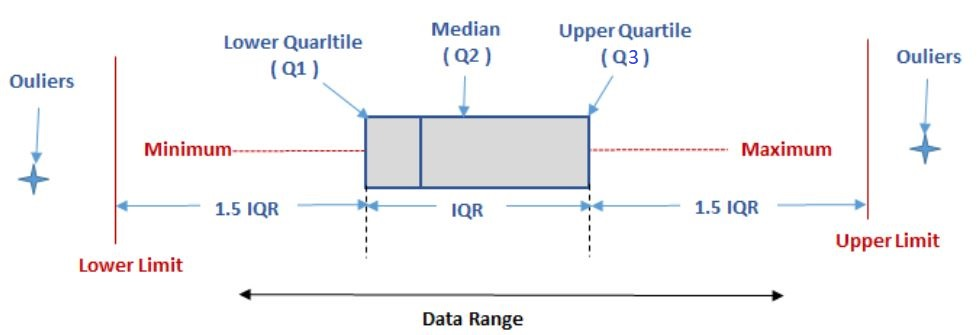
\includegraphics[width=15cm]{boxplot}
	\caption{Box Plot Diagram to identify outliers }
	\label{box}
\end{figure}


The quartiles, Q1 and Q3, are calculated such that the integral of the PDF from $-\infty$ to Q1 equals 0.25 and that of Q3 to $+ \infty$ is 0.75.
Figure \ref{box} depicts a diagram of box plots to detect outliers. In this figure, the factor K is set to 1.5. A point is considered as an outlier if it is not in the range of [Q1 – 1.5 x IQR , Q3 + 1.5 x IQR].\\

\subsubsection{GRUBBS}

Grubbs \cite{grubbs}\cite{stefansky} is an outlier detection algorithm that assumes normality of the distribution. This test detects at most one outlier at a time. It is applied repeatedly until no outliers can be detected. The data is first sorted and then Grubbs tests if the maximum $P_{\max }$ or the minimum $P_{\min }$ data point is an outlier.\\ First, it computes G using:\\
\begin{eqnarray}\label{eq:grubbs}
G_{min}={\frac  {{\bar  {P}}-P_{\min }}{s}} , \text{ and   }
G_{max}={\frac  {P_{\max }-{\bar  {P}}}{s}}
\end{eqnarray}
In Equations (\ref{eq:grubbs}), $\bar{P}$ is the mean of the data points, and $s$ is the standard deviation  computed using:
\begin{eqnarray}\label{std}
s= \sqrt{\frac{1}{N-1}\sum_{i=1}^{N}(P_i-\bar{P})^2}
\end{eqnarray} 
Then, for the two sided test, it compares $G_{min}$  to the threshold using:
\begin{eqnarray}\label{eq:testg}
 G_{min}>{\frac  {N-1}{{\sqrt  {N}}}}{\sqrt  {{\frac  {t_{{\alpha /(2N),N-2}}^{2}}{N-2+t_{{\alpha /(2N),N-2}}^{2}}}}} 
\end{eqnarray}
In (\ref{eq:testg}), $N$ is the number of samples, and $t_{\alpha/(2N),N - 2}$ denotes the upper critical value of the t-distribution with $N - 2$ degrees of freedom and a significance level of $\alpha/(2N)$. If the condition in (\ref{eq:testg}) is satisfied, then $P_{min}$ is identified as an outlier.
Similarily, $G_{max}$, is compared to the threshold in (\ref{eq:testg}) to check if $P_{max}$ is an outlier.
If the one-sided test is used, in equation (\ref{eq:testg}), we replace $\alpha/(2N)$ with $\alpha/N$.
\\
If neither $G_{max}$ nor $G_{min}$ satisfy the in equation (\ref{eq:testg})  are passed, both the min and max are tested for being outliers. First, we compute G using:
\begin{eqnarray}\label{eq:geq}
G={\frac  {P_{\max }-P_{\min }}{s}}.
\end{eqnarray}
Then, we compare G to a threshold and check if:
\begin{eqnarray}\label{eq:geqq}
 G>{\sqrt  {{\frac  {2(N-1)t_{{\alpha /(N(N-1),N-2)}}^{2}}{N-2+t_{{\alpha /(N(N-1),N-2)}}^{2}}}}} 
\end{eqnarray}
In equation (\ref{eq:geqq}), $t_{(\alpha/N(N-1),N-2)} $ denotes the $\alpha/N(N-1)$ percentile of the t-distribution with (N-2) degrees of freedom. If the condition in equation (\ref{eq:geqq}) is satisfied, then both the minimum and the maximum are outliers.\\
\subsubsection{Generalized Extreme Studentized Deviate (GESD)}
GESD \cite{Rosner} is similar to Grubbs and it requires a prior knowledge of the maximum number of outliers to be removed $r$.
To compute GESD, we first compute $R$ , using: 
\begin{eqnarray}
R=\max_{i=1..N}{\frac{|P_i-\bar{P}|}{s}}.
\end{eqnarray}
Then, we remove the data point $P_i$.
Similarly, we compute $R_2$ for the remaining observations (after deleting $P_i$) and delete the $P_j$ that maximizes $R_2$. After repeating the above step $r$ times and computing $R_1, R_2 \dots R_r$, we compare each $R_i$ with $\lambda_i$ and remove the data point that corresponds to the $R_i$ such that $R_i > \lambda_i$ where $\lambda_i$ is computed using:
\begin{eqnarray}
\lambda_i=\frac{t_{(p,N-i-1)}(N-i)}{\sqrt{(N-i-1+t_{(p,N-i-1)}^{2})(N-i-1)}}, \text{ $i=1,...,r$ and, } p=1- \frac{\frac{\alpha}{2}}{N-i+1}
\end{eqnarray}
\subsubsection{Z Score}
Z score \cite{boris} is similar to Grubbs and it assumes normality. First, we compute the zscore of each sample $P_i$ using:
\begin{eqnarray}
Z_{score}(i)=\frac{P_i- \bar{P}}{s},
\end{eqnarray}
The scores are then compared to a constant threshold and the outliers are defined as the data points that have a score larger than the threshold.



\subsubsection{Kimber GESD}
The kimber GESD \cite{kimber} \cite{kimber2} assumes Gamma distribution. It removes the largest observations from the upper end of the sample, starting
with the largest $r$ where $r$ is an input parameters.\\
 for $j = 1, 2, ... , r$ Kimber defines the test statistic $S_j$ by:\\
\begin{eqnarray}
S_j=\frac{P_{N+1-j}}{\sum_{i=1}^{N+1-j}P_i}, \text{ for $j= 1, \dots , r$}
\end{eqnarray}
Then, for $j = r, r- 1, ... , 1$, we check if $ S_j > s_j $, where $s_j=f(j,r,\alpha,N )$ is the appropriate critical value available in Kimber (Figure \ref{kimber}). The largest value of j, say $r*$, for which $S_{r*} > S_{r*}$ declares the upper $r*$ observations as outliers.

\begin{figure}\label{kimber}
	\centering
	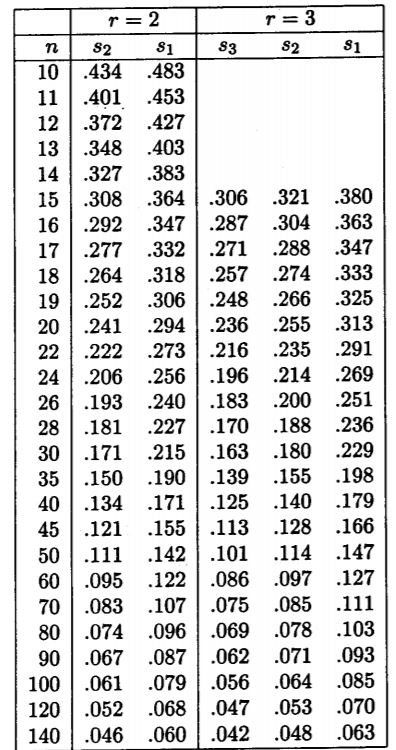
\includegraphics[width=8cm]{kimber}
	\caption{5 \% critical values for Kimber's test for finding up to r upper outliers from
		an exponential distribution }
	
\end{figure}

Table ~\ref{dico} is a summary of the different outlier detection algorithms along with the different  distributions they could be applied to. As it can be seen, Grubbs, GESD and Zscore can be applied to normal and lognormal distributions. On the other hand, Kimber can only be applied to Gamma distributions. Boxplots are the most general and can be applied to any statistical distribution.\\

\begin{table}[h!]
	\centering
	\caption{Applicability of various statistical outlier detection methods to data with the different distribuions}
	\begin{tabular}{|c|c|c|c|c|c |p{3cm}|} 
		\hline
		\textbf{Distribution} & \textbf{GRUBBS} & 	\textbf{GESD} &	\textbf{Kimber} & \textbf{Z Score} &	\textbf{Box Plot}  \\ [0.5ex] 
		\hline\hline
		\textbf{Normal} & x &x& &x&x \\
		\hline
		\textbf{Lognormal} & x &x& &x&x  \\
		\hline
		\textbf{Binomial} & & & & & x  \\
		\hline
		\textbf{Geometric} & & & & & x  \\ 
		\hline
		\textbf{Poisson} & & & & & x  \\
		\hline
		\textbf{Gamma} & & &x & & x  \\
		\hline
	\end{tabular}
	\label{dico}
\end{table}

\subsection{Minimum Volume Ellipsoid}
The Minimum Volume Ellipsoid (MVE) is a common approach used for robust outlier detection in multivariate space  \cite{mve}. It takes subsamples of the dataset and calculates the volume of the ellipsoid that encloses the subsample. The main idea is that outliers increase the volume of the ellipsoid dramatically. Thus, the MVE will correspond to the actual core of the dataset after eliminating outliers. We can consider the samples as ordered by the probability of being an outlier. The first sample is the least probable to be an outlier and the last is the most probable to be an outlier.\\
\indent In the following, we illustrate the MVE with a simple example that includes 10 2-D data points. In figure ~\ref{mve}, different ellipsoids are drawn each time after deleting one outlier at a time. As it can be seen the volume of the ellipsoid has decreased remarkably after deleting the third outlier. In figure ~\ref{mve2}, we plot the evolution of the volume of the ellipsoid as a function of the number of samples each time one sample is identified as outlier and removed. We notice that there is a sudden increase after adding the 8th sample. This increase continues after adding the 9th and the 10th sample. We can conclude that most likely the 8th, 9th and 10th samples are outliers.\\



\begin{figure}
	\centering
	\begin{subfigure}[b]{0.5\textwidth}
		\centering
		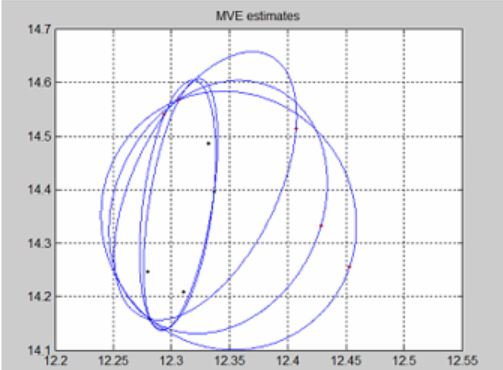
\includegraphics[height=1.9in]{MVEll.JPG}
		\caption{Example Ellipsoids contouring data points Each time after excluding one data point}
		\label{mve}
	\end{subfigure}%
	~ 
	\begin{subfigure}[b]{0.5\textwidth}
		\centering
		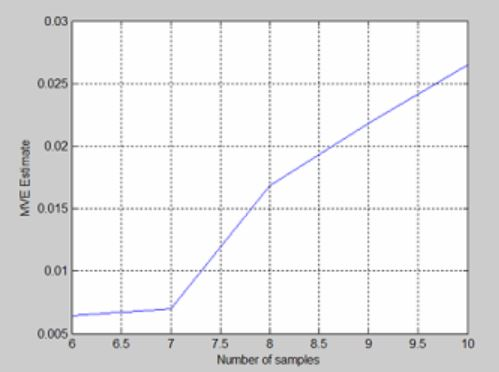
\includegraphics[height=1.9in]{MVEll2.JPG}
		\caption{MVE Estimate (y axis) and sample number (x axis)}
		\label{mve2}
	\end{subfigure}
	\caption{MVE example}
\end{figure}


At the core of the MVE algorithm is the identification of the outlier at each iteration or how to order the samples by their probability of being outliers.
At each iteration, one data sample is chosen as the most probable to be an outlier. We first calculate the Mahalanobis distance matrix of the data points using:
\begin{eqnarray}\label{eq:mve}
M= (X-E) Cov^{-1} (X-E)'
\end{eqnarray}

where $X$ is an ($n \times k$) matrix that include $k$ random features of the $n$ samples. Typically, we choose k=2. In equation (\ref{eq:mve}), $E$ is an $n \times 1$ vector where each component is the mean of the $k$ features, and $cov$ is the covariance matrix of the $n$ samples. Then, we determine the eigenvalues of M and choose the greatest eigenvalue. The data point that has the greatest eigenvalue is the most probable to be an outlier. These steps are repeated at each iteration after removing the identified outliers.

\section{Scaling Methods}
\indent Auto scaling is among the simplest and most common statistical normalization methods. It considers the z score of each data point instead of its initial value along each feature. This method works well when each attribute of the data follows a normal distribution. Since the standard deviation is used as the scaling factor, each normalized feature will have a unit standard deviation and therefore the data can be analyzed on the basis of correlations instead of covariances. Another variation of this method is the Pareto Scaling, where the scaling factor is the square root of the standard deviation \cite{berg:tar}: 
\begin{eqnarray}
P'_{ij}= \frac{P_{ij} - \mu_j}{\sqrt{s_j}}
\end{eqnarray}
Variable Stability Scaling \cite{berg:tar} is another extension of auto-scaling. It uses the coefficient of variation (cv) as a scaling factor. The  cv is defined as the ratio of the standard deviation to the mean, i.e., $ \frac{s}{\mu}$. Using this method, more importance will be attributed to the features that are more stable, i.e. having smaller variation.\\
\indent Range scaling, also known as feature scaling or min-max scaling, is another method that uses the range of the data as a normalization factor. Typically, the range is computed as the difference between the minimal and the maximal value of each feature:
\begin{eqnarray}
P'_{ij}= \frac{P_{ij} - \min_i{P_ij}}{\max_{i}{P_ij}- \min_{i}{P_ij}}
\end{eqnarray}
\section{Data Normalization Methods }
Normalization methods are not restricted to scaling. In fact, several other approaches have been introduced to reduce data variations. These include transformation methods like log transformation, which is usually used to convert multiplicative relations into additive ones to correct heteroscedasticity \cite{keller} and reduce skeweness. A drawback of the log transformation is that it is unable to deal with zero values.  The alternative transformation that overcomes this limitation, while maintaining the positive effects on heteroscedasticity, is the power transformation. A common power transformation method is the one parameter Box-Cox transformation \cite{boxcox}, defined as:
\begin{eqnarray}\label{cox}
y(\lambda)= \left\{
\begin{array}{ll}
\frac{y^{\lambda} -1}{\lambda} & \mbox{, if } \lambda \neq 0 \\
\log \lambda & \mbox{, if }  \lambda = 0 \\
\end{array}
\right.
\end{eqnarray}
Equation (\ref{cox}) holds for $y > 0 $ only. To allow for negative values, the two- parameter Box-Cox transformation defined as:
\begin{eqnarray}\label{gen}
y(\lambda)= \left\{
\begin{array}{ll}
\frac{(y+ \lambda_2)^{\lambda_1} -1}{\lambda_1} & \mbox{, if } \lambda_1 \neq 0 \\
\log (y+\lambda_2) & \mbox{, if }  \lambda_1 = 0 \\
\end{array}
\right.
\end{eqnarray}
could be used. 

In equation (\ref{gen}), $y > -\lambda_2$. The parameters $ \lambda $ , $ \lambda_1$, and $ \lambda_2$ are estimated using the profile likelihood function. A drawback of the power transformation is that it is not able to make multiplicative effects additive.

\subsection{ Quantile Normalization}
Quantile Normalization is typically used in statistics for making two distributions identical. This means that if two data vectors are from the same distribution then the quantile-quantile plot should show a straight diagonal line. Here, we follow the method used in \cite{bolstad:eke:2}, which uses the following transformation: \\
\begin{eqnarray}\label{eq:1}
P_{ij}'= F^{-1}(G(P_{ij}))
\end{eqnarray}
In (\ref{eq:1}), for each feature $i$ and sample $j$, $G$ and $F$ are estimated by the empirical distribution of each feature and the empirical distribution of the averaged sample quantiles respectively.

The quantile method is a general normalization method that can be applied to different fields and applications. 



\subsection{ Cyclic Loess Normalization}
The Cyclic Loess method \cite{dudoit2} is based on fitting a normalization curve to the difference in log expression values (M) versus the average of the log expression values (A) \cite{dudoit} . The normalization curve is fitted using Loess method for local regression \cite{clevland}. Cyclic Loess was first applied to two color channels on the same cDNA array.

For any two arrays $i$ and $j$, with probe intensities $P_{ki}$ and $P_{kj}$ where $k=1, \ldots ,p$ represents the probe, let:
\begin{eqnarray}
& M_k = log_2(P_{ki}/P_{kj}), \\
and &  A_k = \frac{1}{2} log_2(P_{ki} \times P_{kj}) \ 
\end{eqnarray} 
First, an M vs. A plot of the data, where the x-axis is the mean probe expression value of the two arrays ($A_k$) and the y-axis is the difference ($ M_k$) , for $k=1, \ldots ,p$ is generated. 
Next, a smooth Loess curve is fitted to the data.
The outputs of the fitted normalization curve are estimate of $ M_k$, or $\hat{M_k}$. The normalized values for $M_k$ and $P_k$ ($M'_k$ and $P'_k$) are then updated using:

\begin{eqnarray}
& M_k'=M_k - \hat{M_k} , \\
& P'_{ki}= 2^{A_k+\frac{M_k'}{2}} \\
and & P'_{kj}= 2^{A_k-\frac{M_k'}{2}} .
\end{eqnarray} 

An M vs. A plot for normalized data should show a point cloud scattered around the M = 0 axis.  This process can be repeated until useful results are obtained and the probe intensities are adjusted at each iteration.

To handle data sets with  more than two arrays, the above normalization approach can be processed in a pairwise manner. However, this makes this method computationally very intensive.

The Cyclic Loess normalization approach has been adapted to several biological applications such as gene expression array data analysis \cite{ballman}  \cite{hochreiter} and metabolomics data analysis \cite{li}.
A drawback of this method is that it is time consuming. In fact, the time grows in an exponential manner as the size of the array increases. Typically, two or three passes through the complete cycle are required for convergence. 

To overcome this problem, some extensions of the Cyclic Loess normalization such as parallelized implementation were proposed in \cite{ballman}. Other extensions, compare each array to the average of the remaining arrays as in \cite{edwards} and \cite{ballman} instead of comparing arrays in a pairwise manner.

\subsection{ Contrast Based Normalization}
The Contrast based method \cite{astrand:eke} is similar to Cyclic Loess in the way that it also uses an M versus A plot. This method consists of three main steps. First, it changes the basis in which data are logged and transformed using T, an $n \times n$ orthonormal transformation matrix where n is the number of arrays in the data. The 1st row of T is always the 1-vector times $ \sqrt{1/k} $ , and then it follows that the other rows are a set of orthonormal contrast.

Let the first array be the baseline array ($P_b$) and 
$ P= [P_b , P_1 \ldots P_{n-1}] $ be the $k \times n$ data of n arrays and k probes. Let: \\
\begin{eqnarray}
Z= [ P'_b , P'_1 \ldots P'_{n-1}] = log (P) \times T^T \ 
\end{eqnarray} 
be the data in the transformed basis.
The second step in the contrast-based method fits the ($n-1$) normalizing curves in a similar way as in Cyclic Loess, with respect to the remaining baseline array $ P'_b$, and adjusting the data by a smooth transformation. Finally, the normalized data is obtained by transforming back to the original basis and exponentiating. This method was first used for Affymetrix high density oligonucleotide arrays \cite{astrand:eke}. It is slightly faster than Cyclic Loess but still considered as time consuming method.\\